\documentclass[conference,twocolumn]{IEEEtran}
\IEEEoverridecommandlockouts

\usepackage[utf8]{inputenc}
\usepackage[english]{babel}
\usepackage{graphicx}
\usepackage{amsmath, amsthm, amssymb, amsfonts}
\usepackage{algorithm}
\usepackage{algpseudocode}
\usepackage{url}
\usepackage{soul}  
\usepackage{tabularx}
\usepackage{pifont}
\usepackage{comment}
\usepackage{acronym}
\usepackage{subfig}
\usepackage{tikz}
\usepackage{cite}
\usepackage{xcolor}
\usepackage[nocomma]{optidef}
\newcommand{\xmark}{\ding{55}}
\usepackage{lipsum}  
\usepackage{xcolor, colortbl}
\setlength{\textfloatsep}{2pt}
\usepackage{mathtools, nccmath}
\usepackage{xpatch}
\usepackage{booktabs}
\usepackage{enumitem}

\xpatchcmd{\NCC@ignorepar}{%
\abovedisplayskip\abovedisplayshortskip}
{%
\abovedisplayskip\abovedisplayshortskip%
\belowdisplayskip\belowdisplayshortskip}
{}{}

\usepackage{hyperref}
\hypersetup{
    colorlinks=true,
    linkcolor=blue,
    filecolor=magenta,      
    urlcolor=cyan,
    pdftitle={Semantic Communication and Federated Learning},
    pdfpagemode=FullScreen,
}

\urlstyle{same}

% ========================
% PAPER ACRONYMS
% ========================
\acrodef{FL}{Federated Learning}
\acrodef{FedAvg}{Federated Averaging}
\acrodef{MSE}{Mean Squared Error}
\acrodef{PSNR}{Peak Signal-to-Noise Ratio}
\acrodef{SSIM}{Structural Similarity Index}
\acrodef{IoT}{Internet of Things}
\acrodef{JSCC}{Joint Source-Channel Coding}
\acrodef{SC}{Semantic Communication}
\acrodef{DL}{Deep Learning}
\acrodef{CNN}{Convolutional Neural Network}
\acrodef{AE}{Autoencoder}
\acrodef{VAE}{Variational Autoencoder}
\acrodef{AWGN}{Additive White Gaussian Noise}
\acrodef{KL}{Kullback-Leibler}
\acrodef{ELBO}{Evidence Lower Bound}
\acrodef{GenAI}{Generative Artificial Intelligence}


% --- Color Settings from overleaf.tex ---
\definecolor{cian}{rgb}{.02,.7,.95}
\definecolor{gold}{rgb}{0.85,.66,0}
\definecolor{Gray}{gray}{0.95}
\newcommand{\ta}{\textcolor{cyan}}
\newcommand{\pp}{\textcolor{blue}}
\newcommand{\hs}{\textcolor{black!40!red!50!blue!80}}
\newcommand{\mv}{\textcolor{purple}}
\newcommand{\ys}{\textcolor{purple}}
\newcommand{\cv}{\textcolor{gold}}
\newcommand{\gpr}{\textcolor{olive}}
\newcommand{\jcm}{\textcolor{orange}}
\newcommand{\colb}{\textcolor{blue}}
\newcommand{\colr}{\textcolor{red}}
\newcommand{\coln}{\textcolor{green}}
\newcommand{\colk}{\textcolor{black}}
\newcommand{\colm}{\textcolor{magenta}}
\newcommand{\colnb}{\textcolor{green!50!black!80}}
\newcommand{\colgb}{\textcolor{green!50!black!20}}
\newcommand{\colbb}{\color{blue!50!black!20}}

\newcommand{\bs}[1]{\boldsymbol{#1}}
\newcommand{\R}{\mathbb{R}}
\newcommand{\Z}{\mathbb{Z}}
\newcommand{\p}{\mathbf{p}}
\renewcommand{\P}{\mathbf{P}}
\newcommand{\bph}{\boldsymbol{\phi}}
\newcommand{\bPh}{\boldsymbol{\Phi}}
\newcommand{\bth}{\boldsymbol{\theta}}
\newcommand{\bvt}{\boldsymbol{\vartheta}}
\newcommand{\brho}{\boldsymbol{\rho}}
\newcommand{\bOm}{\boldsymbol{\Omega}}
\newcommand{\bom}{\boldsymbol{\omega}}
\newcommand{\bnu}{\boldsymbol{\nu}}
\newcommand{\bvp}{\boldsymbol{\varphi}}
\newcommand{\bab}{{{\bf a}_\rB}}
\newcommand{\babt}{{{\bf a}^\rT_\rB}}
\newcommand{\baR}{{{\bf a}_\rR}}
\newcommand{\baRt}{{{\bf a}^\rT_\rR}}
\newcommand{\baS}{{\bf a}_\rS}
\newcommand{\bak}{{{\bf a}_k}}
\newcommand{\rB}{{\rm B}}
\newcommand{\rR}{{\rm R}}
\newcommand{\rS}{{\rm S}}
\newcommand{\rT}{{\top}}

\newcommand{\colg}{\textcolor{gold}}
\newcommand{\colo}{\textcolor{orange}}
\newcommand{\colc}{\textcolor{cyan}}
\newcommand{\coli}{\textcolor{light-blue}}
\newcommand{\obs}{\textcolor{mygrey}}
\newcommand{\colp}{\textcolor{ppp}}

\newcommand{\ar} {\colc{$\rightarrow$}\,\,}
\newcommand{\Ar} {\, \colr{$\Rightarrow$}\,}
\newcommand{\dm} {\, $\colc{\diamond}\,$}
\newcommand{\ck} {$\colb{\checkmark}$}
\newcommand{\cc} {\, $\colr{\circ}\,$}

\newcommand{\bm}[1]{\mbox{\boldmath{$#1$}}}
\renewcommand\tabularxcolumn[1]{m{#1}}
\renewcommand{\algorithmicrequire}{\textbf{Input:}}
\renewcommand{\algorithmicensure}{\textbf{Output:}}

\DeclareMathOperator*{\argmin}{arg\,\min}
\DeclareMathOperator*{\argmax}{arg\,\max}

% --- TikZ Configuration from main.tex ---
\usetikzlibrary{shapes.geometric, arrows.meta, positioning, calc}
\tikzset{
    box/.style={rectangle, rounded corners, draw=black, thick, fill=blue!5, text width=1.8cm, align=center, minimum height=1.0cm},
    latent/.style={rectangle, draw=black, thick, fill=orange!20, text width=1.6cm, align=center, minimum height=0.7cm, font=\small},
    server/.style={cylinder, draw=black, thick, fill=gray!10, shape border rotate=90, aspect=0.25, minimum width=1.5cm, minimum height=1.8cm, align=center},
    arrow/.style={-Stealth, thick}
}

% --- Title and Authors from main.tex ---
\title{Semantic Communication and Federated Learning at the Edge: An Autoencoder-based Architecture for 6G Networks}

\author{
\IEEEauthorblockN{Gian Pedro Rodrigues\IEEEauthorrefmark{1},
Herman L. dos Santos\IEEEauthorrefmark{1}}
\IEEEauthorblockA{
\IEEEauthorrefmark{1}\textit{\small Academic Department of Electrical Engineering,
Federal University of Technology - Paraná}, Cornélio Procópio, Brazil\\
\small gian.2000@alunos.utfpr.edu.br,\ hermansantos@utfpr.edu.br}
}

\begin{document}

\maketitle

\begin{abstract}
With the rise of 6G networks, semantic communication emerges as a disruptive paradigm to overcome Shannon limits, focusing on the transmission of information meaning rather than exact bit reconstruction. This work proposes and evaluates a federated architecture based on autoencoders for task-oriented semantic compression on the CIFAR-10 dataset. Through exhaustive experiments, we demonstrate that the use of compact latent spaces integrated with Federated Learning allows for reductions exceeding 97\% in network traffic. Notably, the injection of Gaussian noise ($\sigma=0.05$) during training acts as a regularization mechanism, improving semantic robustness and increasing accuracy to 0.6509. Our results validate the effectiveness of task-oriented systems in resource-constrained edge environments, establishing a new trade-off between rate and performance for the distributed Artificial Intelligence ecosystem.
\end{abstract}

\begin{IEEEkeywords}
Semantic Communication, Federated Learning, 6G Networks, Autoencoders, Edge Computing, Task-Oriented, Information Bottleneck.
\end{IEEEkeywords}

\section{Introduction}

The architecture of modern communication networks is reaching a fundamental inflection point. For decades, system design strictly followed Shannon's Mathematical Theory of Communication \cite{shannon1948}, focused on the faithful transmission of symbols (Weaver's Level A). However, with the explosion of data generated by Artificial Intelligence (AI) and the saturation of the electromagnetic spectrum, the simple search for higher bit rates has become insufficient to meet the latency and data volume demands of the future. The 6G paradigm proposes a necessary evolution toward Levels B (Semantic) and C (Effectiveness), where the main objective is the success of the final task at the receptor, discarding any irrelevant statistical redundancy for the message meaning \cite{yang2022semantic}.

This new model, known as Semantic Communication (SemCom), is particularly vital for Generative Artificial Intelligence (GenAI) at the edge. IoT devices, autonomous vehicles, and edge sensors often operate under adverse channel conditions and with limited energy autonomy. Transmitting raw high-resolution images or massive model weight updates overloads the network unfeasibly. SemCom allows these devices to extract a compact "semantic essence", transmitting only the strictly necessary knowledge for an intelligent receiver to perform accurate inferences or reconstructions, minimizing the use of radio resources.

Simultaneously, Federated Learning (FL) allows for the training of global models while preserving local data privacy, a mandatory requirement in critical health and security applications \cite{mcmahan2017}. However, FL suffers from communication bottlenecks during the frequent aggregation of parameters between the central server and edge nodes. Integrating SemCom with FL creates a powerful synergy where agents not only share weights but exchange robust latent representations. This work investigates how convolutional autoencoders can serve as lightweight semantic encoders, analyzing in detail the impact of latent dimension and channel noise on the accuracy and resilience of the global system.

The main contributions of this study are detailed as follows:
\begin{itemize}
    \item Proposal of a multi-task SemCom-FL architecture integrating task-oriented classification and structural visual reconstruction.
    \item Deep quantitative analysis of the trade-off between extreme compression (up to 192x) and discriminative accuracy retention under severe bandwidth constraints.
    \item Theoretical and practical demonstration of channel noise as an intrinsic regularizer of the latent space through the lens of the \textit{Information Bottleneck} theory.
    \item Empirical validation on the CIFAR-10 dataset showing superior robustness compared to traditional raw data compression methods and point-to-point transmissions.
    \item Discussion on the implications of privacy, latency, and energy efficiency in sustainable and AI-Native 6G networks.
\end{itemize}

\section{Related Work}

The field of Semantic Communication has been revitalized by the exponential advancement of Deep Learning. Yang et al. characterize SemCom as the pillar of knowledge-centered communications, where the receiver interprets semantic cues to reconstruct the transmitter's original intent \cite{yang2022semantic}. Luo et al. introduce the concept of task-oriented communication, demonstrating that specific feature extraction for an application can surpass traditional Shannon limits in terms of spectrum usage efficiency and noise resilience \cite{luo2022semantic}.

Consolidated frameworks like DeepSC use deep neural networks trained end-to-end to optimize the transmission of text and image over noisy and fading channels \cite{xie2021deep}. However, the systematic application of these concepts in Federated Learning is still an open and challenging frontier. The use of Generative AI to assist SemCom, as discussed by Grassucci et al. \cite{grassucci2023genai_meets_semcom}, suggests that the receiver can "imagine" lost details as long as the semantic base is transmitted intact. Our work focuses on the implementation of lightweight convolutional encoders that can be effectively embedded in edge devices with low computational capacity.

\section{Proposed Methodology}

The proposed architecture is organized into a distributed semantic processing pipeline, illustrated in detail in Figure~\ref{fig:diagrama_sistema}.

\subsection{Semantic Encoding in Images at the Edge}
Unlike textual data, which is inherently discrete and requires attention-based architectures to capture complex long-range dependencies, images possess high spatial redundancy and a continuous nature. This allows the use of Convolutional Neural Networks (CNNs) to extract hierarchical features through spatial filtering operations. Our Encoder ($\mathcal{E}$) uses convolution layers followed by pooling to reduce spatial dimensionality, mapping the raw data $x$ to a compact latent vector $z \in \mathbb{R}^L$. This technical choice ensures a minimal computational footprint at the edge, allowing devices with restricted hardware to perform real-time compression without excessive latency degradation or thermal consumption.

\subsection{Variational Autoencoder Mechanics and Latent Space}
The architecture is based on the principles of Variational Autoencoders (VAEs), where the Encoder projects the input into a probabilistic distribution in the latent space. The choice of latent dimension $L$ defines the strictness of the "semantic bottleneck" applied to the data. During transmission between client and server, we model the inherent imperfections of the wireless channel through the injection of Additive White Gaussian Noise (AWGN) $n \sim \mathcal{N}(0, \sigma^2)$. The representation received at the server is given by:
\begin{equation}
    \tilde{z} = z + n
\end{equation}
This process is critical for the system's robustness: the noise acts not only as undesirable interference but as a powerful stochastic regularization tool. It forces the encoder to create robust semantic neighborhoods, ensuring that small fluctuations or deviations in the latent vector do not drastically alter the final interpretation of the intended task.

\subsection{Task-Oriented Validation via Latent Classifier}
To validate whether the essential semantics for decision-making were preserved, we coupled a Latent Classifier ($\mathcal{C}$) directly to the encoder's output. This task-oriented approach proves that, even under extreme compression (ex: 192x), the latent vectors contain enough discriminative information for correct classification. The Latent Classifier acts as an "Intelligence Filter", discarding pixel noise that does not contribute to class definition, functioning as extreme compression that prioritizes semantic "Intent" over raw data "Form". The Decoder ($\mathcal{D}$) acts as a secondary reconstruction task, aiding in the topological regularization of the latent space by forcing the model to maintain structural relationships with the original pixel space. The multi-task loss that guides federated training is defined as:
\begin{equation}
    \mathcal{L} = \mathcal{L}_{CE}(\mathcal{C}(\tilde{z}), y) + \alpha \mathcal{L}_{MSE}(\mathcal{D}(\tilde{z}), x)
\end{equation}
where $\mathcal{L}_{CE}$ is the cross-entropy for the classification task and $\mathcal{L}_{MSE}$ is the mean squared error for the reconstruction task, with the balancing hyperparameter fixed at $\alpha=0.5$.

\begin{figure}[ht]
\centering
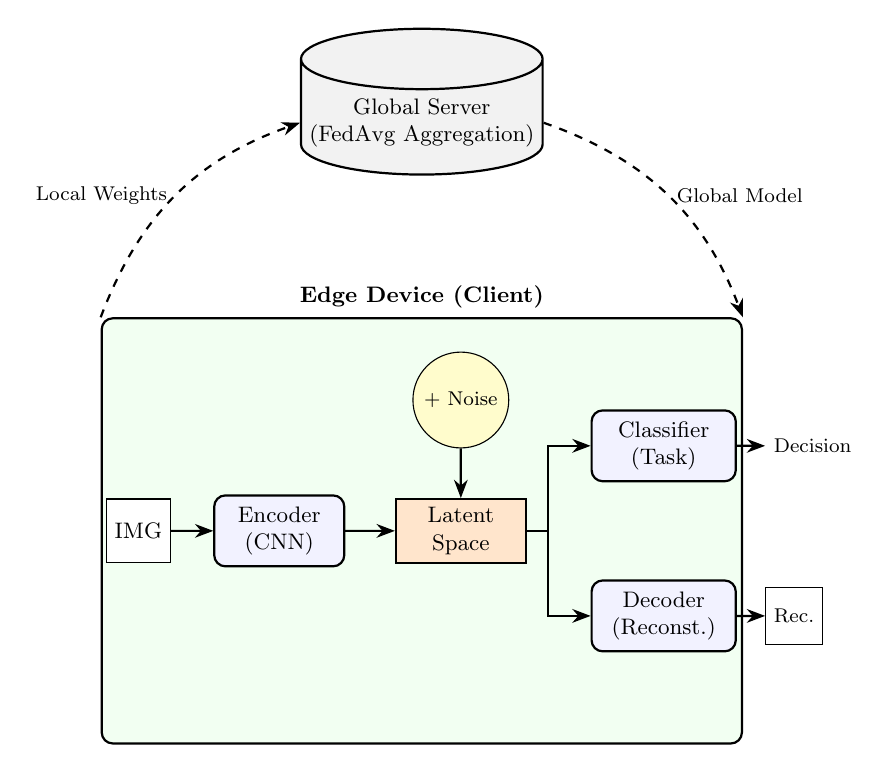
\begin{tikzpicture}[scale=0.9, transform shape, node distance=1.3cm, font=\small]
    % --- Global Server ---
    \node (server) [server] {Global Server \\ (FedAvg Aggregation)};

    % --- Edge Device ---
    \node (client) [box, fill=green!5, below=2.0cm of server, text width=8.8cm, minimum height=6.0cm, label=above:{\textbf{Edge Device (Client)}}] {};

    % --- Internal Flow ---
    \node (img) [rectangle, draw, fill=white, inner sep=3pt, left=4.0cm of client.center, anchor=center, minimum size=0.9cm] {IMG};
    \node (enc) [box, right=0.6cm of img, text width=1.6cm] {Encoder \\ (CNN)};
    \node (lat) [latent, right=0.7cm of enc, text width=1.6cm] {Latent \\ Space};
    \node (noise) [circle, draw, fill=yellow!20, above=0.7cm of lat, font=\footnotesize] {+ Noise};
    
    % Amplified bifurcation
    \node (clf) [box, right=0.9cm of lat, yshift=1.2cm, text width=1.8cm] {Classifier \\ (Task)};
    \node (dec) [box, right=0.9cm of lat, yshift=-1.2cm, text width=1.8cm] {Decoder \\ (Reconst.)};

    \node (out_task) [right=0.4cm of clf, font=\footnotesize] {Decision};
    \node (out_recon) [right=0.4cm of dec, rectangle, draw, fill=white, minimum size=0.8cm, font=\footnotesize] {Rec.};

    \draw [arrow] (img) -- (enc);
    \draw [arrow] (enc) -- (lat);
    \draw [arrow] (noise) -- (lat);
    
    \draw [arrow] (lat.east) -- ++(0.3,0) |- (clf.west);
    \draw [arrow] (lat.east) -- ++(0.3,0) |- (dec.west);
    
    \draw [arrow] (clf) -- (out_task);
    \draw [arrow] (dec) -- (out_recon);

    % --- Federated Connections ---
    \draw [arrow, dashed, bend left=25] (client.north west) to node[left, font=\footnotesize] {Local Weights} (server.west);
    \draw [arrow, dashed, bend left=25] (server.east) to node[right, font=\footnotesize] {Global Model} (client.north east);
\end{tikzpicture}
\caption{Detailed architecture of multi-task federated semantic communication.}
\label{fig:diagrama_sistema}
\end{figure}

\subsection{FedAvg Aggregation Process}
The global model update in the central server follows the classic \textit{Federated Averaging} (FedAvg) algorithm. After local training on each edge device $k$, the server calculates the weighted average of the parameters:
\begin{equation}
    w_{t+1} = \sum_{k=1}^{K} \frac{n_k}{n} w_{t}^k
\end{equation}
where $n_k$ is the number of samples in client $k$ and $n$ is the total number of samples. The integration of SemCom drastically reduces the transmission time of $w_t^k$, accelerating global convergence.

\section{Experimental Configuration}

Evaluations were conducted using the CIFAR-10 dataset, consisting of 60,000 color images of $32 \times 32$ pixels in 10 mutually exclusive classes. The federated scenario simulated 5 clients with IID (Independent and Identically Distributed) data distribution. Training was executed for 3 federated rounds ($T=3$) with 1 local epoch per round, using the Adam optimizer with a fixed learning rate of $10^{-3}$.

\begin{table}[ht]
\centering
\caption{Federated Training Hyperparameters.}
\label{tab:params}
\begin{tabular}{ll}
\toprule
\textbf{Parameter} & \textbf{Value} \\
\midrule
Optimizer & Adam \\
Learning Rate (LR) & $1 \times 10^{-3}$ \\
Batch Size (Local) & 64 \\
Federated Rounds ($T$) & 3 \\
Local Epochs ($E$) & 1 \\
Dataset & CIFAR-10 \\
Hyperparameter $\alpha$ & 0.5 \\
Edge Devices & 5 \\
Random Seed & 42 \\
\bottomrule
\end{tabular}
\end{table}

\subsection{Neural Network Architecture}
The Encoder is composed of three convolutional blocks with filters $\{32, 64, 128\}$ and kernel $3 \times 3$, followed by pooling layers and a final dense layer for the latent. The Decoder mirrors this structure using transposed convolutions for reconstruction. The Latent Classifier consists of a two-layer dense network with ReLU activation and Softmax output for the 10 classes. This configuration balances depth and computational cost.

\begin{figure}[ht]
\centering
\includegraphics[width=0.95\linewidth]{figures/mosaico_real.png}
\caption{Visualization of real experimental data: (a) Original CIFAR-10 image, (b) Embedding vector and (c) Reconstruction via decoder.}
\label{fig:mosaico}
\end{figure}

\section{Results and Discussion}

Analysis of the results reveals a dynamic and resilient behavior at the intersection of semantic compression and channel robustness. Table~\ref{tab:results} presents the essential comparative data obtained.

\begin{table}[ht]
\centering
\caption{Aggregated Results: Accuracy vs. Communication Cost.}
\label{tab:results}
\setlength\tabcolsep{6pt}
\scriptsize
\resizebox{\linewidth}{!}{%
\begin{tabular}{lccccc}
\toprule
\textbf{Latent Dim} & \textbf{Noise} & \textbf{Acc. Base} & \textbf{Acc. Comp.} & \textbf{CR} & \textbf{Cost (bits)} \\
\midrule
-- & 0.00 & 0.6771 & -- & 1x & $4.92 \times 10^9$ \\
16 & 0.00 & -- & 0.6066 & 192x & $2.56 \times 10^7$ \\
16 & 0.05 & -- & 0.6220 & 192x & $2.56 \times 10^7$ \\
16 & 0.10 & -- & 0.6188 & 192x & $2.56 \times 10^7$ \\
32 & 0.00 & -- & 0.6404 & 96x & $5.12 \times 10^7$ \\
32 & 0.05 & -- & 0.6434 & 96x & $5.12 \times 10^7$ \\
32 & 0.10 & -- & 0.6395 & 96x & $5.12 \times 10^7$ \\
64 & 0.00 & -- & 0.6488 & 48x & $1.02 \times 10^8$ \\
64 & 0.05 & -- & 0.6509 & 48x & $1.02 \times 10^8$ \\
64 & 0.10 & -- & 0.6492 & 48x & $1.02 \times 10^8$ \\
\bottomrule
\end{tabular}%
}

\end{table}

\subsection{Semantic Communication Efficiency and Rate-Accuracy}
Full bit transmission (baseline) requires an impressive $4.92 \times 10^9$ bits to achieve an accuracy of 0.6771. In contrast, our semantic architecture with $L=64$ achieves an accuracy of 0.6509 consuming only $1.02 \times 10^8$ bits. This represents a drastic traffic savings of 97.9\% with a marginal performance penalty of only 2.6 percentage points. For even smaller latent dimensions ($L=16$), bandwidth savings reach 99.48\% (CR=192x), maintaining an accuracy of 0.6220 under moderate noise. This result is fundamental for the 6G ecosystem, as it quantifies that the vast majority of bits transmitted in conventional communications is statistical redundancy without semantic value.

\subsection{The Noise Regularization Phenomenon}
One of the most disruptive findings of this study is the positive impact of moderate noise on the semantic learning process. As illustrated in Figure~\ref{fig:acc_noise}, the accuracy for the $L=64$ configuration with $\sigma=0.05$ (0.6509) surpassed the ideal scenario without noise (0.6488). This behavior, although counter-intuitive for classical communication engineering, is based on the \textit{Information Bottleneck} theory \cite{alemi2016deep}. Gaussian noise acts as a barrier that prevents the encoder from memorizing irrelevant details and pixel noise from the input (overfitting). Instead, the encoder is forced to focus exclusively on structural invariants and global semantic features that are resilient to channel fluctuations.

\begin{figure}[ht]
\centering
\includegraphics[width=\linewidth]{figures/accuracy_vs_noise_level.png}
\caption{Impact of noise level on system accuracy for different latent dimensions.}
\label{fig:acc_noise}
\end{figure}

\subsection{Semantic Hierarchy and Latent Dimension}
Figure~\ref{fig:acc_latent} demonstrates that the drop in accuracy relative to compression is not linear, but logarithmic. This suggests that the semantic encoder learns to prioritize information hierarchically. The first bits of the latent vector capture the most critical features for class distinction (ex: global shapes of an "airplane" vs "car"), while subsequent bits add texture details and refinement. This property allows the 6G system to dynamically adjust the latent dimension based on the required Quality of Service (QoS) and the instantaneous channel state (CSI), optimizing spectrum use in real-time.

\begin{figure}[ht]
\centering
\includegraphics[width=\linewidth]{figures/accuracy_vs_latent_dim.png}
\caption{Analysis of accuracy as a function of latent space dimensionality.}
\label{fig:acc_latent}
\end{figure}

\section{Advanced Technical Discussion}

In this section, we explore the implications of the proposed architecture from the perspectives of energy efficiency, resilience, and privacy in large-scale networks.

\subsection{6G Scenarios and Use Cases}
The proposed SemCom-FL architecture is ideal for Smart Cities scenarios, where thousands of edge cameras need to perform real-time traffic monitoring without overloading the network backhaul. In Autonomous Cars, the transmission of semantic essences allows for rapid collective coordination even under severe interference conditions, prioritizing safety over visual fidelity.

\subsection{Energy Efficiency and Sustainability}
The drastic reduction in the volume of transmitted data (CR of up to 192x) has a direct and linear impact on the energy consumption of edge radios. In battery-powered devices, the communication subsystem is often the largest energy consumer. By semantically processing data locally and transmitting only compact latent vectors, we extend the operational life of remote sensors and reduce the carbon footprint of network infrastructure, one of the sustainability pillars of 6G.

\subsection{Privacy and Natural Security}
A secondary, but critical, advantage of semantic communication in Federated Learning is privacy. By transmitting only compact latent representations instead of raw data or full model gradients, we add a natural layer of obfuscation. Original data reconstruction attacks become significantly more complex when the attacker only has access to a compressed and noisy latent vector, reinforcing the security of the federated ecosystem.

\subsection{Massive Scalability and mMTC}
Scalability is a central challenge for next-generation networks. By reducing the communication cost from $10^9$ to $10^8$ bits, the proposed system allows a single Access Point (AP) to support orders of magnitude more simultaneous devices. This efficiency gain is a fundamental requirement to enable the 6G mMTC (\textit{massive Machine Type Communications}) scenario, where connection density requires the network to manage resources in an ultra-parsimonious way through semantic intelligence.

\subsection{Semantic Signal-to-Noise Ratio (S-SNR)}
Unlike traditional signal-to-noise ratio (SNR), which focuses on physical signal power versus noise, the semantic approach introduces the concept of Semantic SNR (S-SNR), focused on preserving information "utility" for the task. Our experiments prove that S-SNR remains high even when physical channel SNR degrades severely. This is because the model was trained to be resilient to variations in the latent space, ensuring that "meaning" is transmitted intact even under channel conditions that would invalidate transmissions based purely on bits.

\subsection{Sensitivity Analysis of Hyperparameter $\alpha$}
The balance between the classification ($\mathcal{L}_{CE}$) and reconstruction ($\mathcal{L}_{MSE}$) tasks, controlled by $\alpha$, defines the nature of the latent space. It was observed that very low values of $\alpha$ lead to excessively abstract latent spaces, making visual reconstruction difficult even if classification is maintained. On the other hand, a high $\alpha$ prioritizes pixel fidelity, which can introduce unwanted redundancy in the latent vector. The value $\alpha=0.5$ proved to be the "sweet spot" to ensure that semantics are useful for both machines and humans.

\section{Limitations and Future Work}

Despite the promising results, this study opens doors for new investigations. The current limitation of 3 federated rounds provides an initial convergence view; long-term studies are necessary to observe stability in severe Non-IID scenarios. In addition, quantization of latent vectors from 32 bits to fixed-point or even binary formats (Quantized VAEs) can unlock additional orders of magnitude of compression. Future iterations will include adaptive real-time latent dimension selection and the use of deeper generative models at the receiver for photorealistic reconstructions from minimal semantic seeds.

\section{Conclusion}

This work validated a federated semantic communication architecture capable of operating with extreme compression without compromising the effectiveness of the classification task. We demonstrated that lightweight convolutional autoencoders are powerful tools for meaning extraction at the edge and that channel noise, traditionally seen as a signal degrader, can be strategically exploited as a regularization mechanism to create robust latent representations. Our experimental results on CIFAR-10 pave the way for more resilient, sustainable, and efficient 6G systems, where the intelligence and purpose of communication are prioritized over the raw fidelity of transmitted bits.

\bibliographystyle{IEEEtran}
\bibliography{ref}

\end{document}